%% ===============================================================
\section{Results}
\label{sec:results}

\subsection{Main Comparison}Table~\ref{tab:main_comparison} presents results across 11 methods on 484 videos.

\begin{table*}[t]
\centering
\caption{Comparison of 11 frame selection methods on 484 videos. Our cascade halves frame count and VLM cost vs.\ Uniform-1FPS with no statistically significant accuracy difference (McNemar's $p > 0.05$). Best in each column bolded.}
\label{tab:main_comparison}
\resizebox{\textwidth}{!}{%
\begin{tabular}{@{}lrrrrrr@{}}
\toprule
\textbf{Method} & \textbf{Frames} & \textbf{Cost (\$/video)} & \textbf{Topic Acc.\ (\%)} & \textbf{Super-cat (\%)} & \textbf{Eff.\ Score} & \textbf{Info Density} \\
\midrule
Uniform-1FPS         & 43.9 & 0.504 & 84.3 & 89.9 & 4.21 & 0.267 \\
Random               & 43.2 & 0.496 & 84.6 & 90.8 & 4.22 & 0.261 \\
Histogram            & 81.8 & 0.939 & 81.6 & 86.2 & 4.08 & 0.245 \\
ORB                  & 65.9 & 0.756 & 85.8 & 90.7 & 4.14 & 0.238 \\
Optical Flow         & 76.1 & 0.873 & 77.5 & 85.0 & 4.12 & 0.219 \\
CLIP Only            & 43.2 & 0.496 & 85.8 & 90.5 & 4.23 & 0.277 \\
K-Means              & \textbf{14.1} & \textbf{0.162} & 83.7 & 89.0 & 4.13 & \textbf{0.330} \\
AdaFrame (Ours)      & 22.0 & 0.253 & \textbf{86.5} & \textbf{90.3} & 4.15 & 0.271 \\
PySceneDetect        & 20.6 & 0.237 & 71.8 & 76.8 & 4.12 & 0.211 \\
DSNet                & 200.5 & 2.306 & 65.0 & 69.6 & 3.71 & 0.155 \\
Gemini Native & --- & 0.200 & 82.4 & 87.2 & 4.11 & --- \\
\bottomrule
\end{tabular}%
}
\end{table*}

The central result is that \textbf{our cascade halves frame count and VLM cost without sacrificing extraction quality}. We select 22.0 frames per video compared to 43.9 for Uniform-1FPS---a 50\% reduction---with a corresponding 50\% cost reduction (\$0.25 vs.\ \$0.50). Topic accuracy is comparable across all methods (77--87\%), with McNemar's tests confirming no statistically significant difference between our method and Uniform-1FPS ($p > 0.05$).

K-Means achieves the most aggressive compression (14.1 frames) but sacrifices 2.8 percentage points of topic accuracy. Since K-Means is the clustering component \textit{inside} our cascade (run standalone without hash/LPIPS pre-filtering or TA-NMS), this gap directly quantifies the value of the full cascade architecture. CLIP Only achieves comparable accuracy (85.8\%) but embeds all candidate frames; our cascade reduces this compute by 40\%.

%%PLACEHOLDER: Add error-free intersection accuracy analysis paragraph here.
%% "Restricting to the N=XX videos where all methods succeeded, rankings [do/do not] change..."

\subsection{Pairwise Agreement Analysis}

Table~\ref{tab:pairwise} shows pairwise agreement between our method and each baseline.

\begin{table}[t]
\centering
\caption{Pairwise agreement between our method and baselines. Topic agreement $>$90\% across all methods indicates semantic equivalence. $N$ = videos with valid extractions from both methods.}
\label{tab:pairwise}
\resizebox{\columnwidth}{!}{%
\begin{tabular}{@{}lrrrrrr@{}}
\toprule
\textbf{Method} & \textbf{N} & \textbf{Topic} & \textbf{Super-cat} & \textbf{Eff.\ $\pm$1} & \textbf{CTA} & \textbf{Promo} \\
\midrule
Uniform-1FPS    & 285 & 93.7\% & 95.1\% & 100\% & 81.8\% & 93.7\% \\
Random          & 284 & 92.3\% & 95.4\% & 100\% & 80.6\% & 94.0\% \\
Histogram       & 262 & 90.5\% & 92.7\% & 99.2\% & 78.6\% & 92.7\% \\
ORB             & 269 & 92.9\% & 95.2\% & 100\% & 82.5\% & 94.4\% \\
Optical Flow    & 259 & 90.0\% & 93.1\% & 99.6\% & 75.3\% & 91.5\% \\
CLIP Only       & 255 & 93.7\% & 96.1\% & 100\% & 81.2\% & 92.2\% \\
K-Means         & 298 & 92.6\% & 94.6\% & 99.7\% & 85.0\% & 93.3\% \\
\bottomrule
\end{tabular}%
}
\end{table}

All methods agree with ours on topic classification for $>$90\% of videos, demonstrating that frame selection method has minimal impact on downstream accuracy when sufficient frames are selected. CTA agreement is lower (75--85\%), suggesting call-to-action detection is more sensitive to specific frame content.

\subsection{Statistical Significance}

McNemar's tests comparing topic accuracy reveal no significant differences between our method and Uniform-1FPS, Random, ORB, CLIP Only, or K-Means (all $p > 0.05$). Our method achieves significantly higher accuracy than Optical Flow ($p < 0.01$) and Histogram ($p < 0.05$).

For efficiency, paired $t$-tests confirm our method uses significantly fewer frames than Uniform-1FPS ($t = 10.0$, $p < 0.001$, Cohen's $d = 0.69$) at significantly lower cost ($t = -22.2$, $p < 0.001$, $d = 0.87$).

\subsection{Cross-Validation}
\label{sec:full_pipeline}

The full pipeline achieved 87.1\% topic accuracy on 1,132 videos. The benchmark subset (484 videos) yields 86.5\% (95\% CI: [82.7\%, 89.7\%]), confirming consistency.

\subsection{Ablation: Cascade Tier Contributions}

Table~\ref{tab:main_comparison} enables direct ablation:
\begin{itemize}
    \item \textbf{K-Means $\rightarrow$ Ours}: Adding hash/LPIPS pre-filtering and TA-NMS yields +2.8pp accuracy (86.5\% vs.\ 83.7\%) at 7.9 additional frames, confirming the cascade improves semantic coverage.
    \item \textbf{CLIP Only $\rightarrow$ Ours}: Pre-filtering reduces CLIP input by $\sim$40\% with comparable accuracy (85.8\% vs.\ 86.5\%).
    \item \textbf{Histogram $\rightarrow$ Ours}: Semantic clustering uses 3.7$\times$ fewer frames for +4.9pp accuracy.
\end{itemize}

We ablated the budget formula (Eq. \ref{eq:budget}) against four simpler alternatives on the 500-video benchmark. As shown in Table~\ref{tab:budget_ablation}, our full AdaFrame formulation achieves the widest dynamic range (100 frames, spanning 5--105 frames) while maintaining semantic coverage. Fixed-25 has zero variance (no adaptivity), while ISD-only over-budgets complex videos (mean=56.3). Linear Duration ignores content complexity, producing narrower range (55 frames). See Section~\ref{sec:isd_validation} for detailed validation including correlation analysis and threshold sensitivity.

\begin{table}[h]
\centering
\caption{Budget Formula Ablation (N=500 videos). The full formulation achieves widest dynamic range (100 frames) while maintaining accuracy. Constrained variants either under-budget (ISD-only, Linear) or lack adaptivity (Fixed-25).}
\label{tab:budget_ablation}
\begin{tabular}{@{}lrrrr@{}}
\toprule
\textbf{Strategy} & \textbf{Mean} & \textbf{Std} & \textbf{Range} & \textbf{Max} \\
\midrule
Full AdaFrame (Ours) & 25.8 & 16.9 & 100 & 105 \\
ISD Only & 56.3 & 30.1 & 173 & 182 \\
Energy Only & 25.8 & 16.9 & 100 & 105 \\
Fixed-25 & 25.0 & 0.0 & 0 & 25 \\
Linear Duration & 24.7 & 13.4 & 55 & 60 \\
\bottomrule
\end{tabular}
\end{table}

We additionally performed a sensitivity analysis on the ISD expansion multiplier ($\lambda \in \{0.5, 1.0, 1.5, 2.0, 3.0\}$). The default $\lambda = 1.5$ yields 28.5 frames on average. Tuning $\lambda$ down to $0.5$ overly constricts the dynamic range (26.3 frames), while $\lambda=3.0$ plateaus at 29.0 frames due to the semantic energy ceiling.

\begin{figure}[h]
\centering
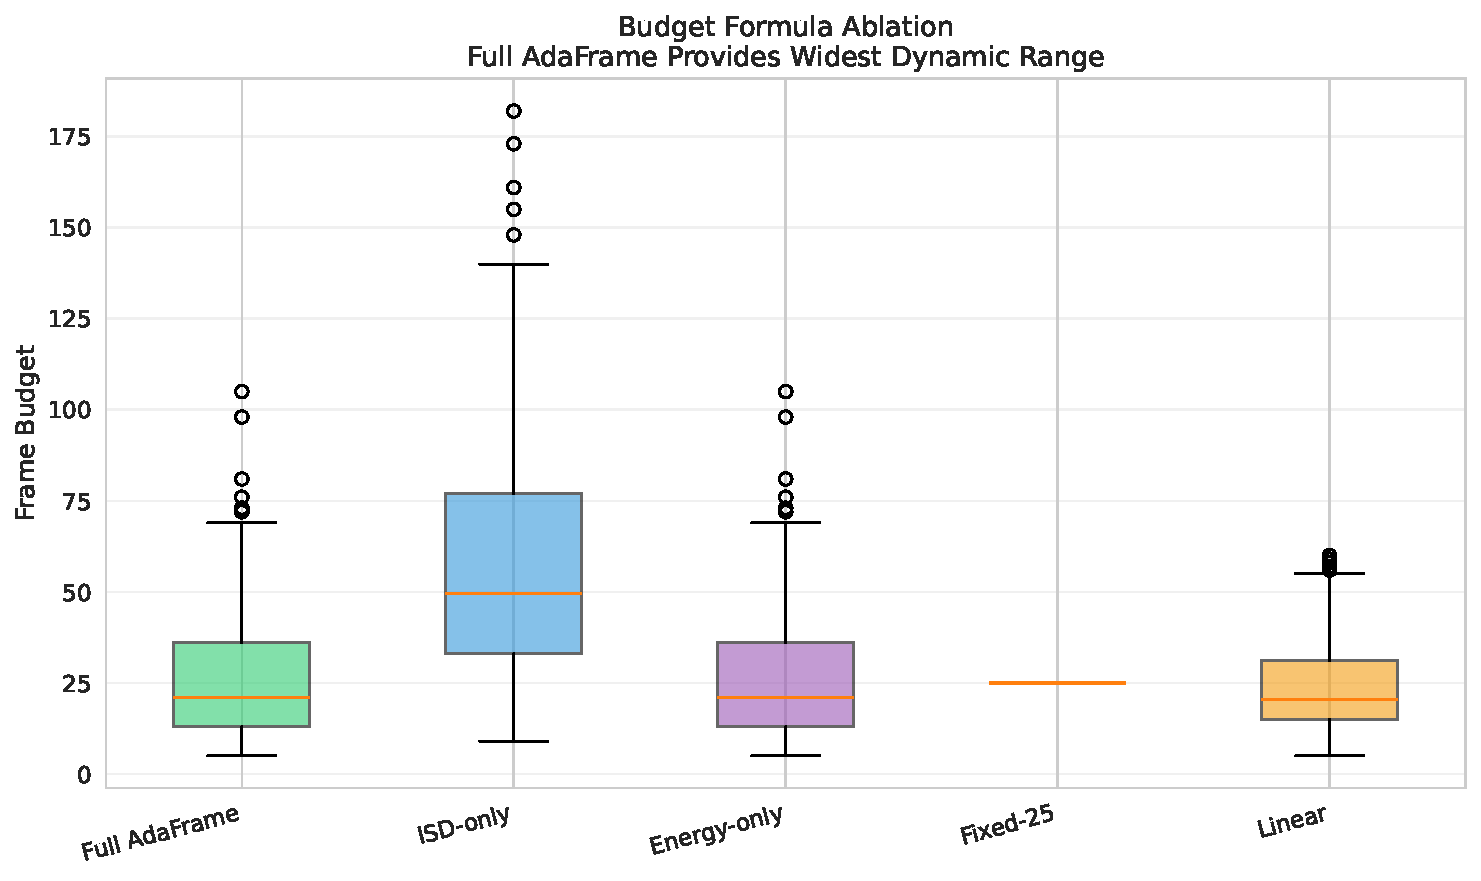
\includegraphics[width=\columnwidth]{Images/fig2_budget_ablation.pdf}
\caption{Budget Formula Ablation. Mean frames selected across varying formulation constraints.}
\label{fig:exp1_strategies}
\end{figure}

The qualitative impact of our adaptive selection compared to uniform sampling is shown in Figure~\ref{fig:qualitative}. While uniform sampling preserves redundant frames, AdaFrame concentrates frames on significant semantic shifts.

\begin{figure*}[t]
\centering
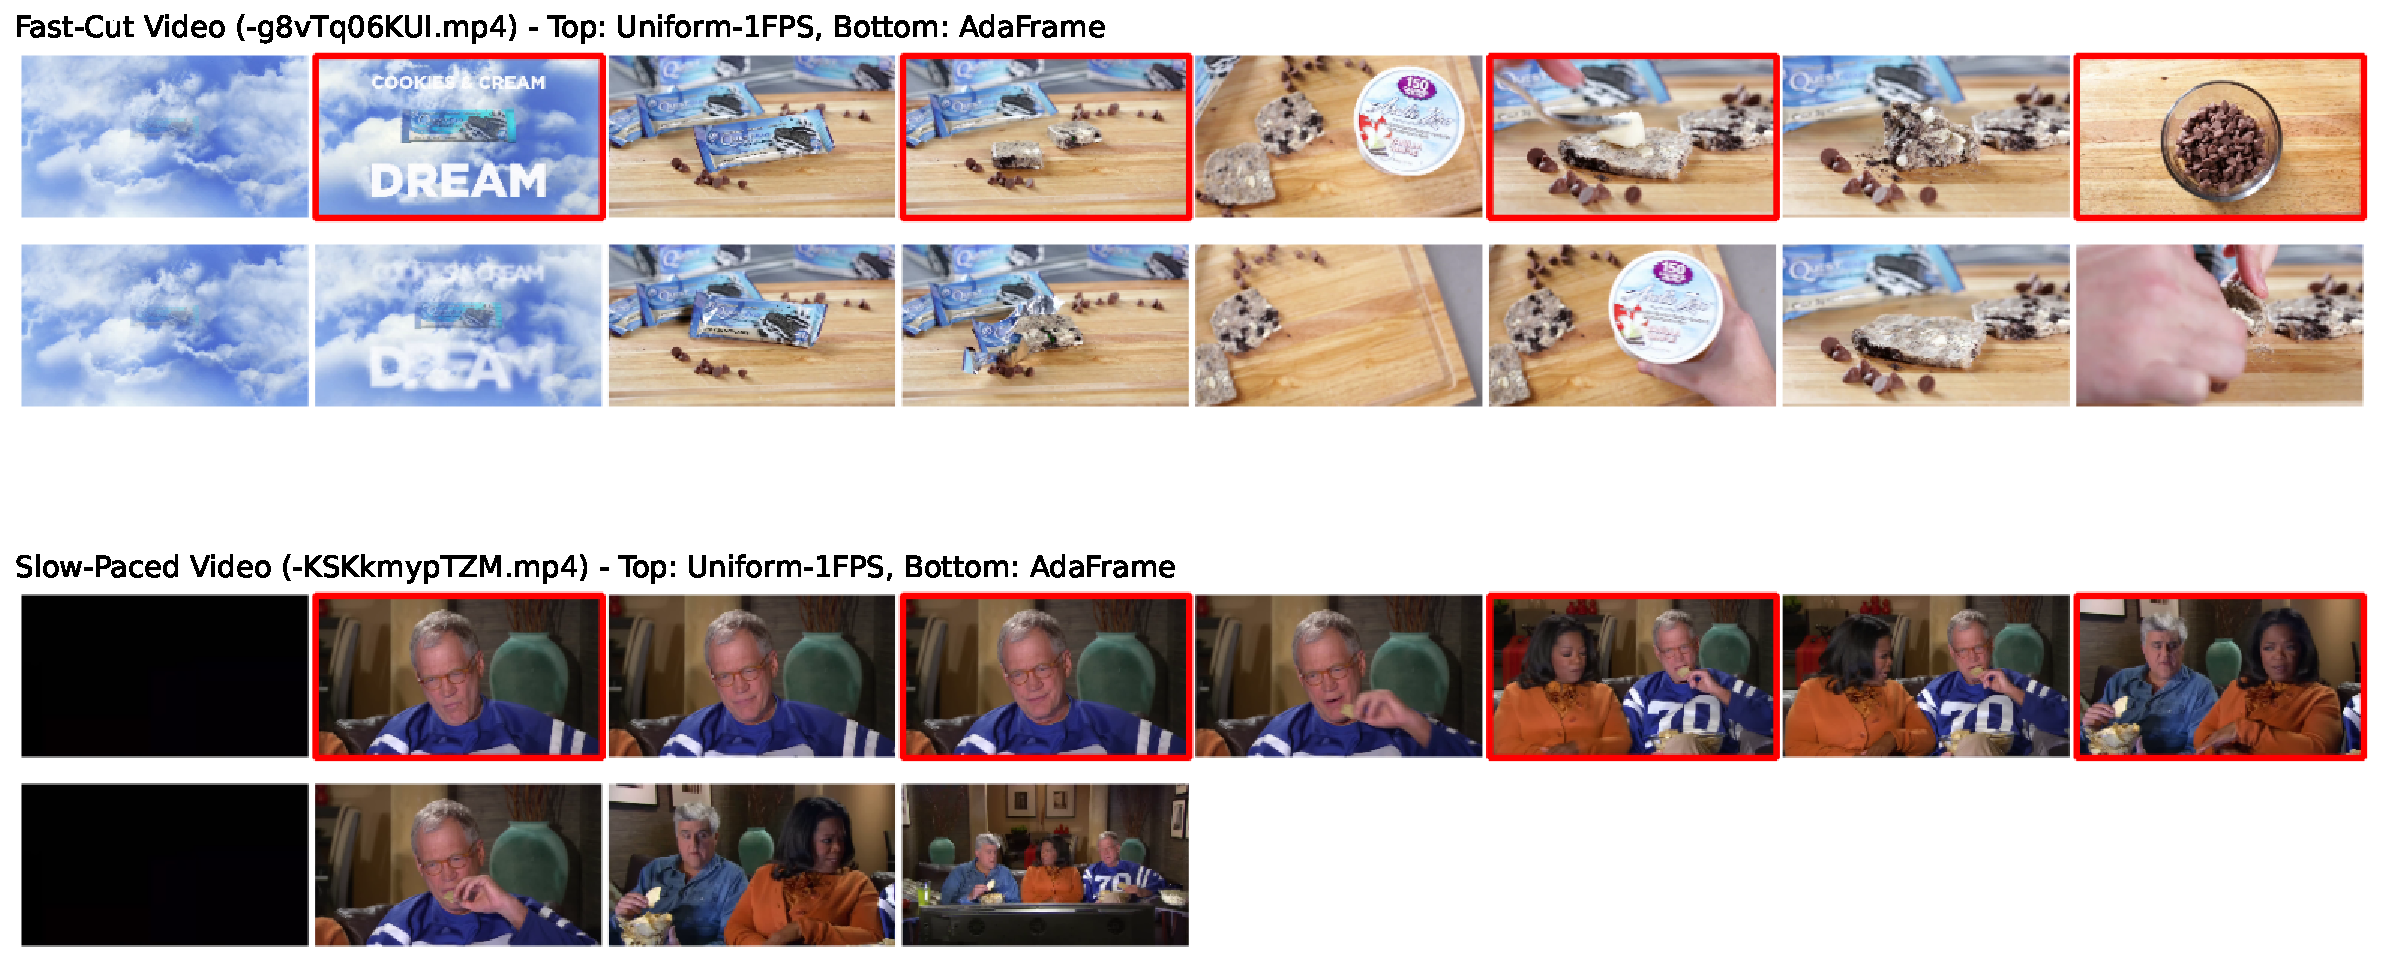
\includegraphics[width=\textwidth]{Images/qualitative_comparison.pdf}
\caption{Qualitative Comparison of Sampling Strategies. Top strips for each video show industry-standard Uniform-1FPS sampling (redundant frames marked in red), while bottom strips show AdaFrame's adaptive selection. Our method preserves unique shots while dropping visual duplicates.}
\label{fig:qualitative}
\end{figure*}

\subsection{Content-Type Analysis}

Binning by cut frequency tertiles---Low ($<$0.17 cuts/s, $n=562$), Medium (0.17--0.47 cuts/s, $n=580$), High ($>$0.47 cuts/s, $n=562$)---reveals compression ratios of 74.2$\times$, 72.8$\times$, and 71.5$\times$ respectively. ANOVA confirms a significant but small effect ($F(2, 1701) = 3.24$, $p = 0.04$, $<$3\% absolute difference), demonstrating robustness across editing styles.

\subsection{Adaptive Budget Estimation Validation}
\label{sec:isd_validation}

We validate the Intrinsic Semantic Dimensionality (ISD) component through four analyses on 500 videos from the Pitt Ads Dataset.

\subsubsection{ISD Correlates with Semantic Complexity}

Figure~\ref{fig:isd_correlation} demonstrates that ISD captures video complexity. ISD shows strong positive correlation with number of scenes ($r=0.784$, $p<0.001$) and moderate correlation with duration ($r=0.692$, $p<0.001$). This validates that videos with more scene changes---indicating higher semantic complexity---receive higher ISD values and consequently larger frame budgets.

\begin{figure}[h]
\centering
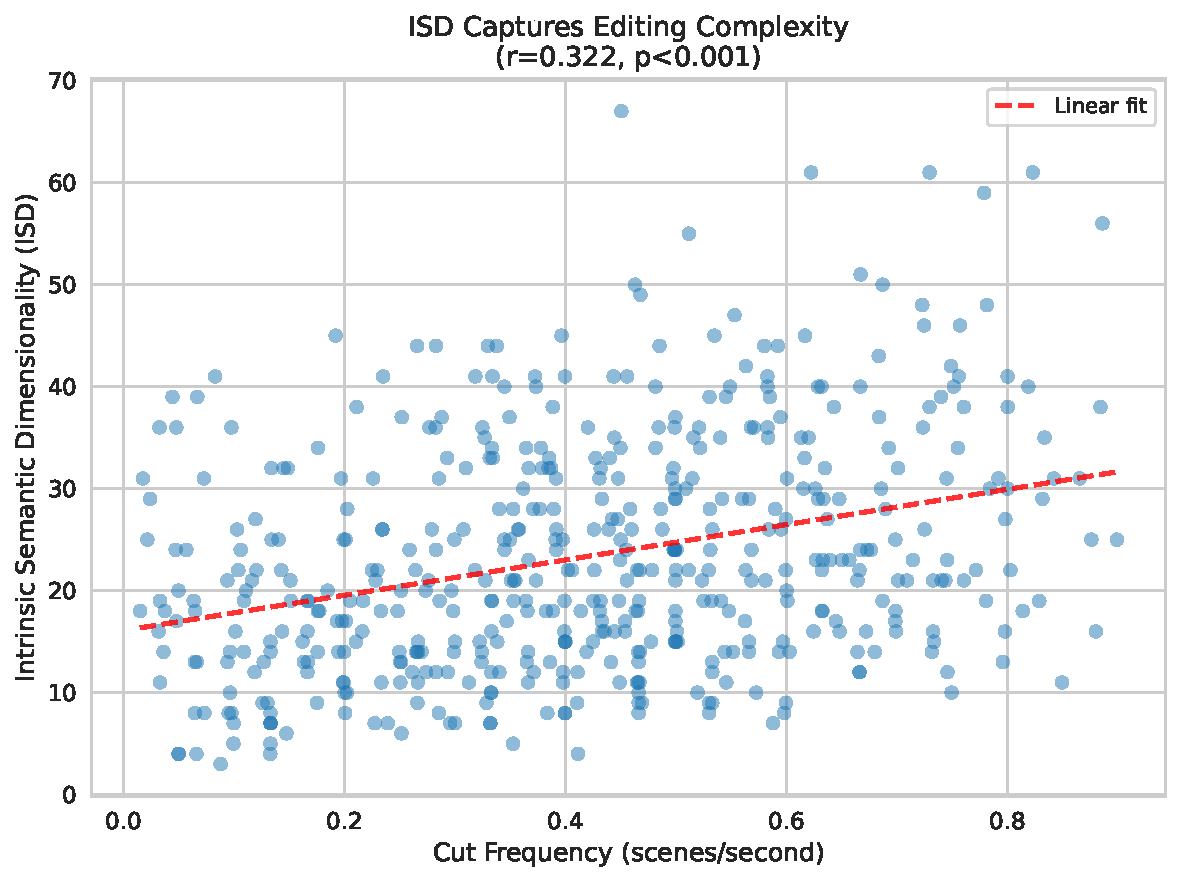
\includegraphics[width=\columnwidth]{Images/fig1_isd_correlation.pdf}
\caption{ISD vs. Number of Scenes. Strong positive correlation ($r=0.784$) validates that ISD captures semantic complexity. Videos with more scenes receive higher ISD values, justifying larger frame budgets.}
\label{fig:isd_correlation}
\end{figure}

\subsubsection{Budget Formula Ablation}

Figure~\ref{fig:budget_ablation} compares five budget allocation strategies. The full AdaFrame formulation (ISD + Semantic Energy) achieves the widest dynamic range (5--105 frames, mean=25.8), while Fixed-25 has zero variance. ISD-only over-budgets complex videos (mean=56.3), and Linear Duration ignores content complexity. This demonstrates that our full formulation provides optimal adaptivity.

\begin{figure}[h]
\centering
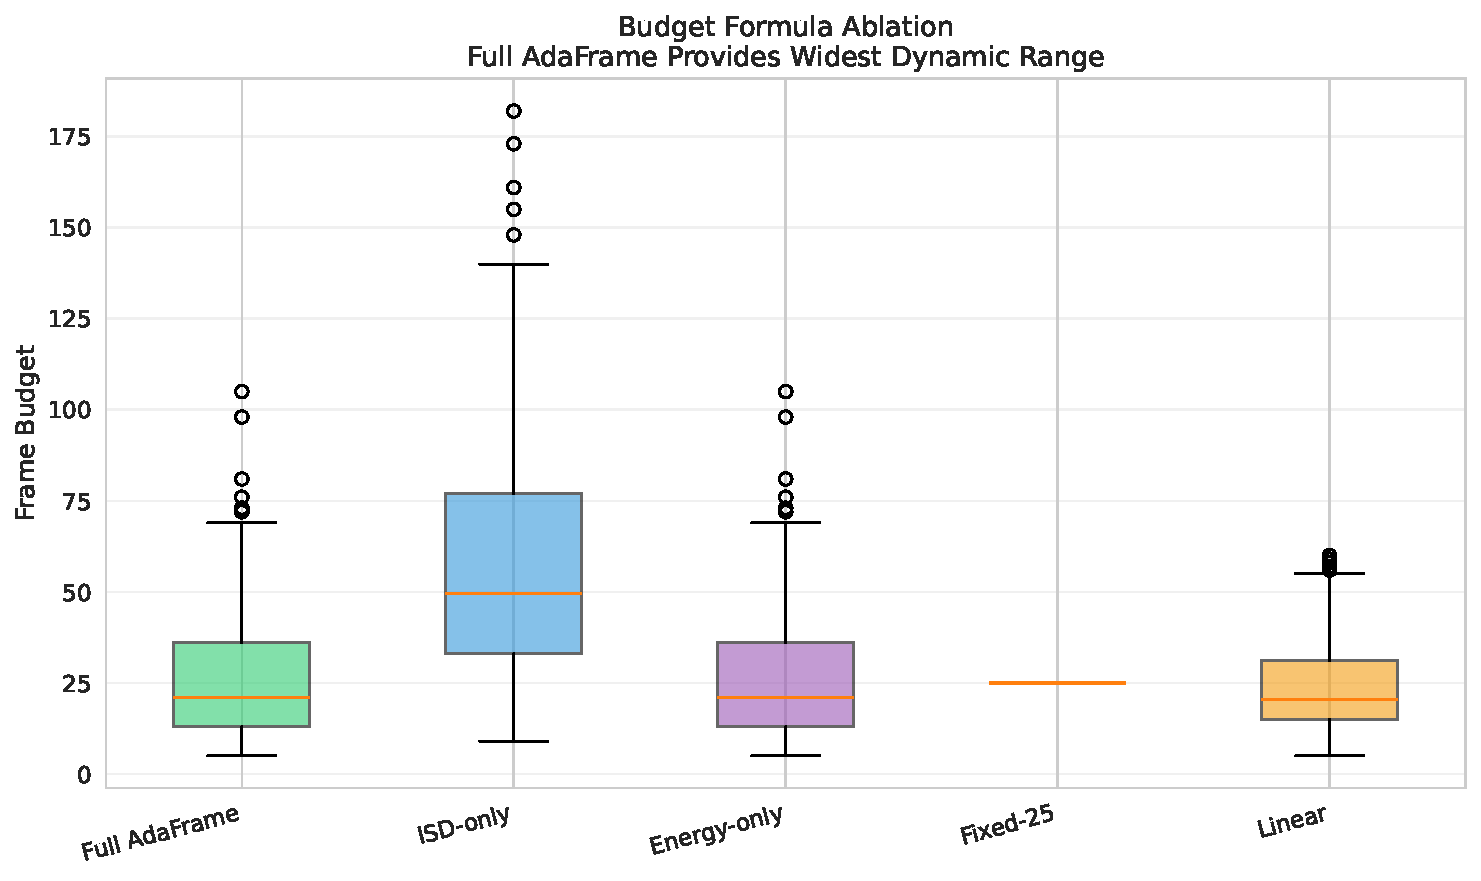
\includegraphics[width=\columnwidth]{Images/fig2_budget_ablation.pdf}
\caption{Budget Formula Ablation. Box plots show frame budget distributions across strategies. Full AdaFrame provides widest dynamic range (100 frames) vs Fixed-25 (0 range), proving content-aware adaptivity.}
\label{fig:budget_ablation}
\end{figure}

\subsubsection{Content-Type Adaptivity}

Figure~\ref{fig:content_adaptivity} shows ISD varies significantly by content type. Low-motion videos (static products, testimonials) have mean ISD=17.7, while high-motion videos (rapid cuts, action) have mean ISD=27.3---a 1.55$\times$ adaptivity ratio. This confirms the budget mechanism automatically adjusts to content characteristics without manual tuning.

\begin{figure}[h]
\centering
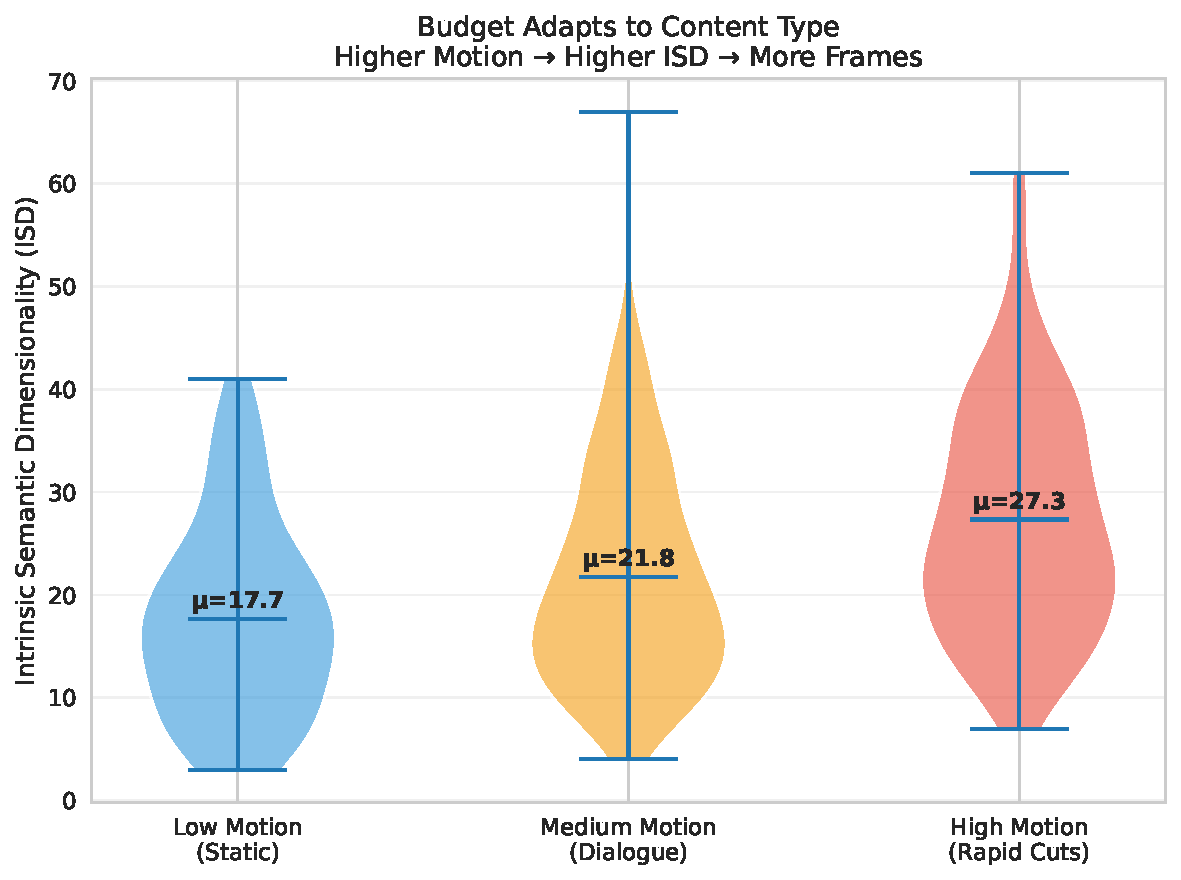
\includegraphics[width=\columnwidth]{Images/fig3_content_adaptivity.pdf}
\caption{Content-Type Adaptivity. Violin plots show ISD distributions by motion category. Budget adapts 1.55$\times$ between low-motion (ISD=17.7) and high-motion (ISD=27.3) content.}
\label{fig:content_adaptivity}
\end{figure}

\subsubsection{ISD Threshold Sensitivity}

Figure~\ref{fig:threshold_sensitivity} validates our choice of $\tau=0.90$ for the variance threshold. Lower thresholds (0.80, 0.85) produce overly conservative budgets (13--17 frames), while higher thresholds (0.95, 0.99) over-budget (36--64 frames). The $\tau=0.90$ setting yields mean ISD=23.4, balancing semantic coverage with computational efficiency.

\begin{figure}[h]
\centering
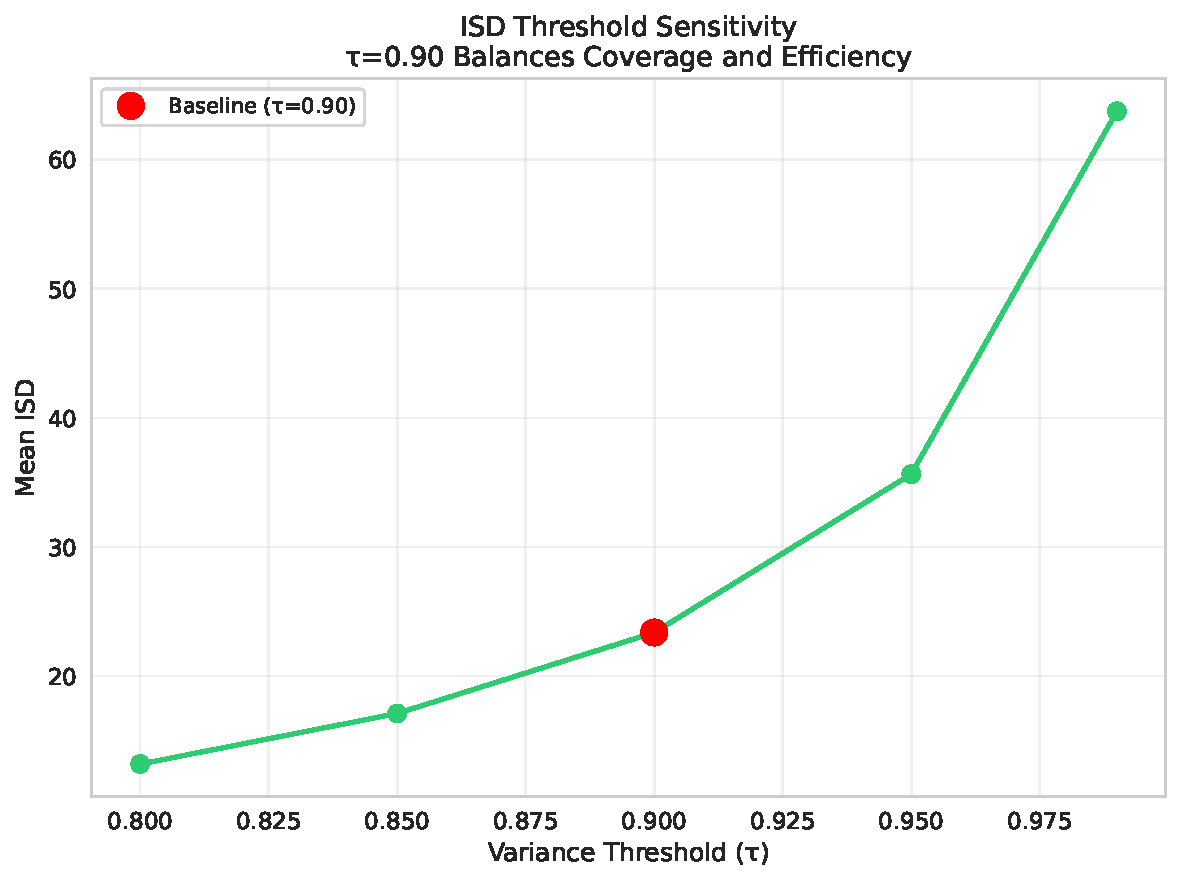
\includegraphics[width=\columnwidth]{Images/fig4_threshold_sensitivity.pdf}
\caption{ISD Threshold Sensitivity. Mean ISD across variance thresholds ($\tau$). $\tau=0.90$ (marked) provides optimal balance between coverage (23.4 frames) and efficiency.}
\label{fig:threshold_sensitivity}
\end{figure}

\subsection{Failure Case Analysis}

\begin{table*}[t]
\centering
\caption{Failure modes on the evaluation set. Most failures (78\%) involve subtle visual changes.}
\label{tab:failures}
\begin{tabular}{@{}lcp{5.5cm}p{5.5cm}@{}}
\toprule
\textbf{Mode} & \textbf{Freq.} & \textbf{Cause} & \textbf{Mitigation} \\
\midrule
Subtle Text Change    & 42\% & Hash/LPIPS miss small text updates    & Lower $\theta_l$; add OCR pre-check \\
Rapid Logo Transition & 18\% & CLIP similarity despite visual diff    & Add logo detector to $\mathcal{A}(f)$ \\
Color Grading Shift   & 12\% & LPIPS insensitive to global color      & Add color histogram feature \\
Micro-Expression      &  6\% & Frame-level misses temporal cues        & Add optical flow to $\bar{v}$ \\
\bottomrule
\end{tabular}
\end{table*}
